%% \documentclass[twocolumn]{article}
\documentclass[pre,twocolumn,twoside,byrevtex,superscriptaddress]{revtex4}

\usepackage{amsmath}
\usepackage{amssymb}
\usepackage{url}
\usepackage{graphicx}
\usepackage{listings,color}
\usepackage{setspace}

\lstset{language=matlab,
        basicstyle=\ttfamily\scriptsize\singlespacing,
        keywordstyle=\color{blue},
        stringstyle=\color{red},
        commentstyle=\color{green},
        morecomment=[l][\color{magenta}]{\#},
        frame=L,
        xleftmargin=\parindent,
        numbersep=5pt,
        breaklines=true,
        breakatwhitespace=false,
        escapeinside={\%*}{*)},
}

\setlength{\parindent}{0cm}

\setlength{\parskip}{1mm}

\begin{document}

%% \twocolumn[
%%   \begin{@twocolumnfalse} 

%%     \title{\vspace{-2cm}Homework 4: Counterprop}
%%     \author{Andy Reagan}

%%     \maketitle

%%   \end{@twocolumnfalse}
%% ]

\title{\vspace{-2cm}Homework 6: GRNN}
\author{Andy Reagan}

\begin{abstract}
I code and discuss a Generalized Regression Nueral Network (GRNN) as described in Specht in his 1991 paper.
\end{abstract}

\maketitle

\section{Introduction}

Brought forth by Specht, the GRNN is a powerful interpolating nueral network \cite{specht1991a}.

%% \begin{figure}
%%  \centering
%%   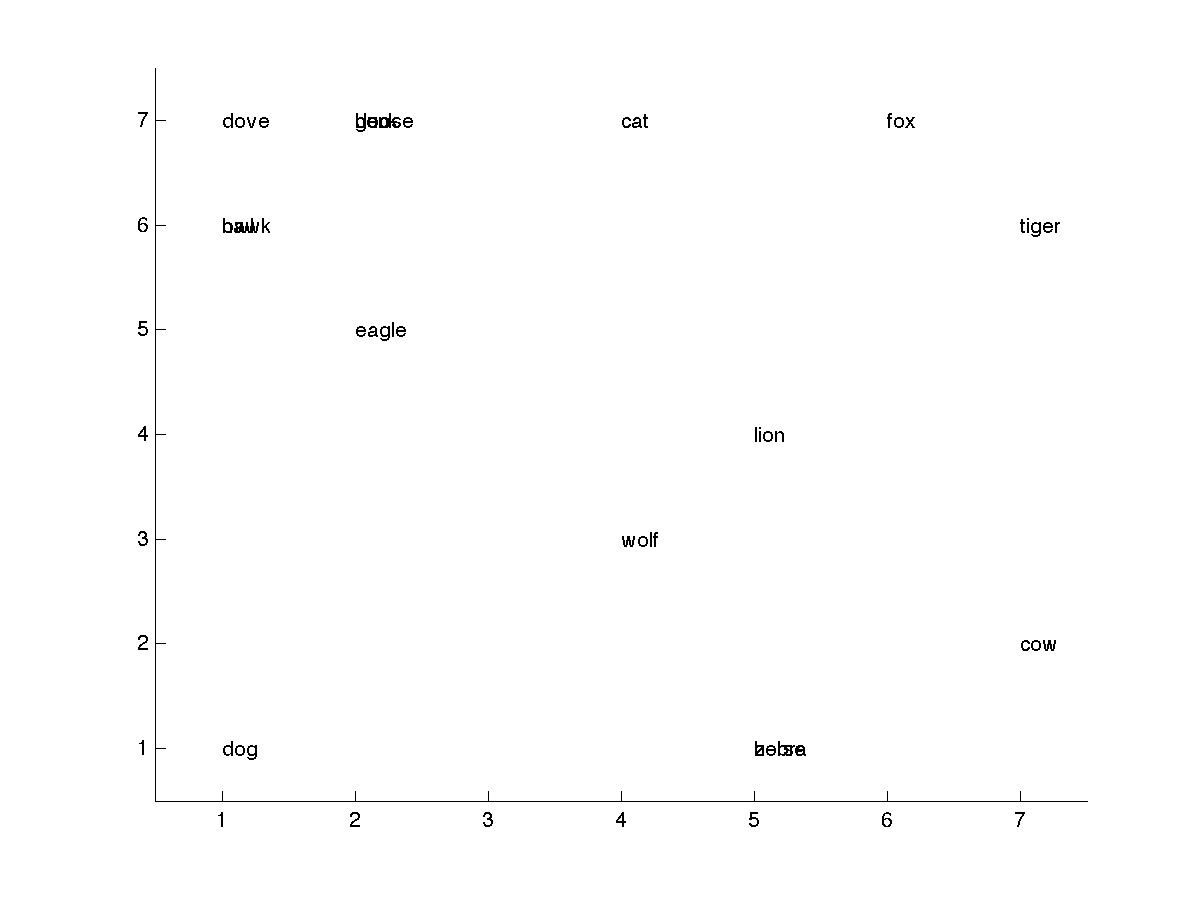
\includegraphics[width=0.48\textwidth]{../figures/animals-layout.png}
%%   \label{fig:1}
%%   \caption{Labels for different animals plotted over their closest Kohonen node.
%% The nodes are laid out on a square grid, which is like the topology of the network, which uses a Von Neumann neighborhood.
%% Some animals have the same attributes, and got plotted in the same place!}
%% \end{figure}



\section{Methods}



\section{Results}



\bibliographystyle{chicago}
\bibliography{writeup}

\clearpage
\pagebreak
\onecolumngrid

    \section*{Full code}

    %% \lstinputlisting{GRNN_andy_driver.m}

%% \clearpage
%% \pagebreak

%%     \section*{Extra figures}

%%     %% \begin{figure}
%%     %%   \centering
%%     %%   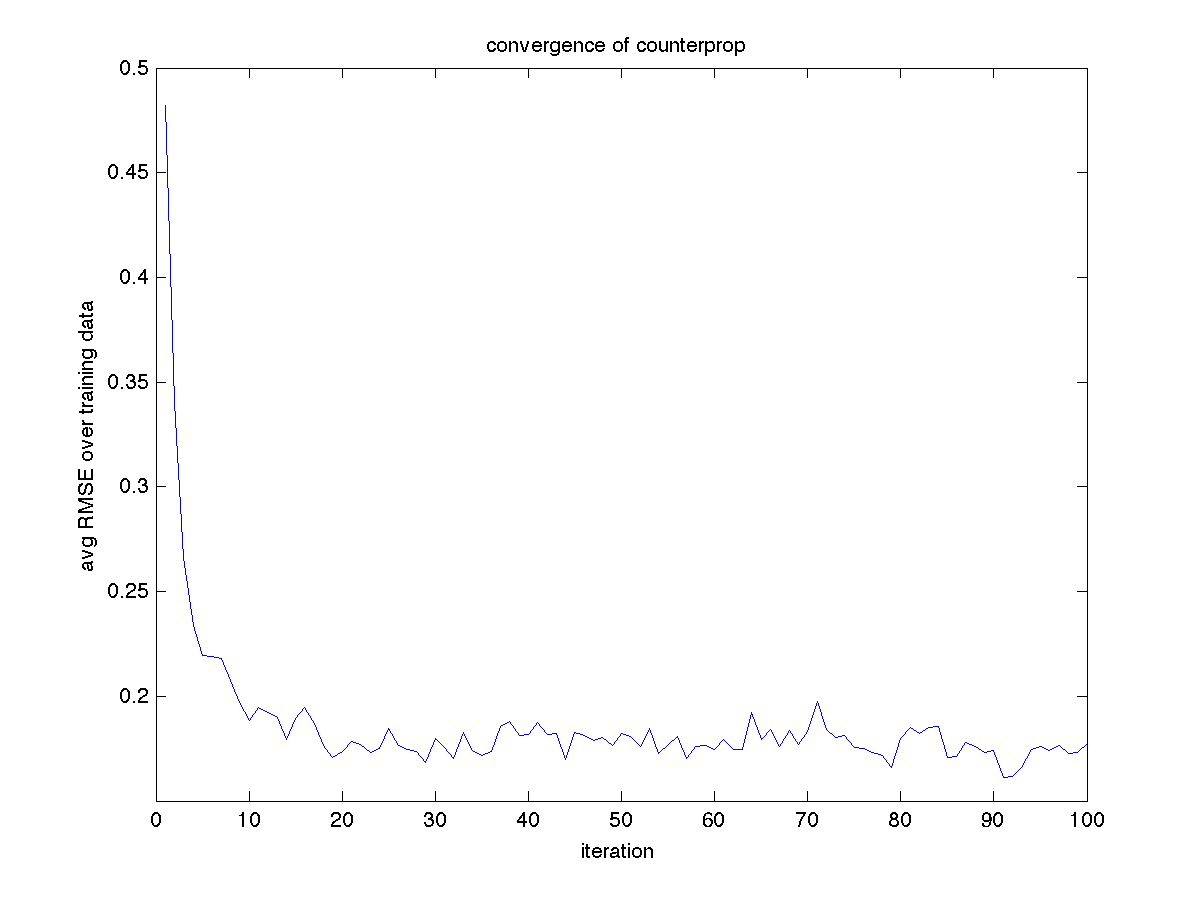
\includegraphics[width=0.68\textwidth]{111.png}
%%     %%   \label{fig:1}
%%     %%   \caption{Basic convergence test.}
%%     %% \end{figure}

\end{document}
